\documentclass[../HAFiscal]{subfiles}
\begin{document}

\FloatBarrier
\section{Robustness}
\label{sec:robustness}

In this section we analyze how sensitive our results are to some of the parameters in the model. In particular, we focus on the degree of risk aversion and the interest rate. These parameters respectively influence the incentive to save through the strength of a precautionary saving motive and through the returns obtained on saving. The aim is to alter these incentives while maintaining the requirement that the distributions of liquid wealth in each education group matches the distribution in the data. Our procedure is therefore to alter the parameter of interest and to repeat the estimation of the degree of `splurge' spending in consumption and the distributions of discount factors within each education group. We then compute new results using these updated estimates. 

\subsection{Increasing risk aversion} 
\label{sec:robust_gamma} 

In our baseline calibration consumers are have log-preferences over consumption and hence have a risk aversion of $\gamma=1$. It is quite common in macroeconomic models to use higher degrees of risk aversion, so here we investigate how alternative values of $\gamma$ would influence our results. The first thing to note is that, in our model, consumers are ex-ante heterogeneous in that they belong to different education groups and have different discount factors. Heterogeneity in discount factors is thus the only device we use to obtain a model where the distribution of liquid wealth can match the data. Thus, when we change risk aversion, the change applies equally to all different types. For the model to continue to match liquid wealth, the distribution of discount factors within each education group must be reestimated. 

\subsubsection{Estimating discount factor distributions with higher risk aversion}
\label{sec:robust_gamma_estim}

Table~\ref{tab:robustness_gamma} displays the values we obtain for the splurge and the discount factor distributions when we increase $\gamma$ to $2$ and $3$. The first result is that the splurge is not very sensitive to the degree of risk aversion. The splurge controls the degree of spending that consumers do before considering the trade-off involved in optimally allocating spending over time. Thus a parameter that affects that trade-off does not have a big influence on that parameter. 

\begin{table}[t]
\begin{center}
\begin{tabular}{lc|cccccc} 
	\toprule
	& & \multicolumn{2}{c}{Dropout} & \multicolumn{2}{c}{Highschool} & \multicolumn{2}{c}{College} \\ \midrule 
	& Splurge & $\beta$ & $\nabla$ & $\beta$ & $\nabla$ & $\beta$ & $\nabla$ \\ \midrule 
	$\gamma = 1.0$ (baseline) & 0.314 & 0.799 & 0.228 & 0.937 & 0.066 & 0.985 & 0.012 \\ 
	$\gamma = 2.0$ & 0.307 & 0.551 & $0.5^*$ & 0.834 & 0.181 & 0.963 & 0.036 \\
	$\gamma = 3.0$ & 0.304 & 0.350 & $0.35^*$ & 0.671 & 0.364 & 0.917 & 0.087 
	\\ \bottomrule 
\end{tabular}
\end{center}
\caption{Estimates of the Splurge and $(\beta,\nabla)$ for each education group for different values of risk aversion, $\gamma$. $*$ indicates a value that is fixed in the estimation --- this is necessary in some cases to prevent the estimation procedure from trying negative values for the discount factor of some type.}
\label{tab:robustness_gamma}
\end{table}

Furthermore, the last four columns show results for the Highschool and College groups that are quite intuitive. Increasing risk aversion for all types within an education group makes the precautionary saving motive stronger for all consumers in that group. Ceteris paribus consumers would then increase the amount of liquid wealth they accumulate, and the median liquid wealth to permanent income ratio for the education group would increase. As the higher risk aversion applies equally to all types within the education group this would also decrease the concentration of liquid wealth within the group. Hence, when we reestimate the discount factor distributions for the Highschool and College groups to fit the same liquid wealth distribution as before, we obtain distributions centered on lower values of beta that are more spread out. Thus the updated discount factor distribution counteracts these two effects. The top right and bottom left panels of Figure~\ref{fig:LorenzPts_robustness} show that with the reestimated discount factor distributions the model continues to match the distribution of liquid wealth as well as in the baseline calibration.\footnote{The median liquid wealth to permanent income ratios in Panel~B of Table~\ref{tab:estimBetas} are also matched in these estimations.} 

For the Dropout group the results are different however. For that group the median liquid wealth to permanent income ratio is very low at only $4.64$, and the liquid wealth distribution is very concentrated. The highest 20 percent of consumers in this group hold $96.4$ percent of the liquid wealth in the Dropout education group. With increased risk aversion for all types within the group, the model cannot match this wealth distribution. The reason is that to fit such a low value of median liquid wealth to permanent income when the strength of the precautionary saving motive increases, we need a discount factor distribution centered around a very low value. But this value places an upper bound on how spread out the discount factor distribution can be, since we can not allow any types in the model to have a negative discount factor. Hence, when the distribution is centered on a low value of $\beta$ it cannot be dispersed enough to match the high concentration of liquid wealth in the Dropout group in the data. 

We deal with this issue by focusing on matching the median liquid wealth to permanent income ratio. Our approach is to fix the value of the spread of the discount factor distribution, $\nabla$, and then estimate the center of the distribution, $\beta$ to match this ratio. The aim is to fix a value of $\nabla$ as high as possible without running into negative values for the discount factor of the least patient type. We end up fixing values of $\nabla=0.5$ when $\gamma=2$ and $\nabla=0.35$ when $\gamma=3$. The columns for the Dropout group in Table~\ref{tab:robustness_gamma} then show that we obtain values for $\beta$ in line with the intuition discussed above: higher risk aversion and a stronger precautionary saving motive leads to discount factor distributions centered around lower values of $\beta$ in order to continue matching the median liquid wealth to permanent income ratio. The upper left panel of Figure~\ref{fig:LorenzPts_robustness} shows that we then cannot obtain distributions of liquid wealth that are as concentrated as in the data. This follows since we cannot allow negative values for the discount factor of any type, and the increased incentive to save affects all the types in the Dropout group making the liquid wealth distribution less concentrated. 

TODO: add discussion of potentially allowing heterogeneity in risk aversions? 

\begin{figure}[th]
\begin{center}
	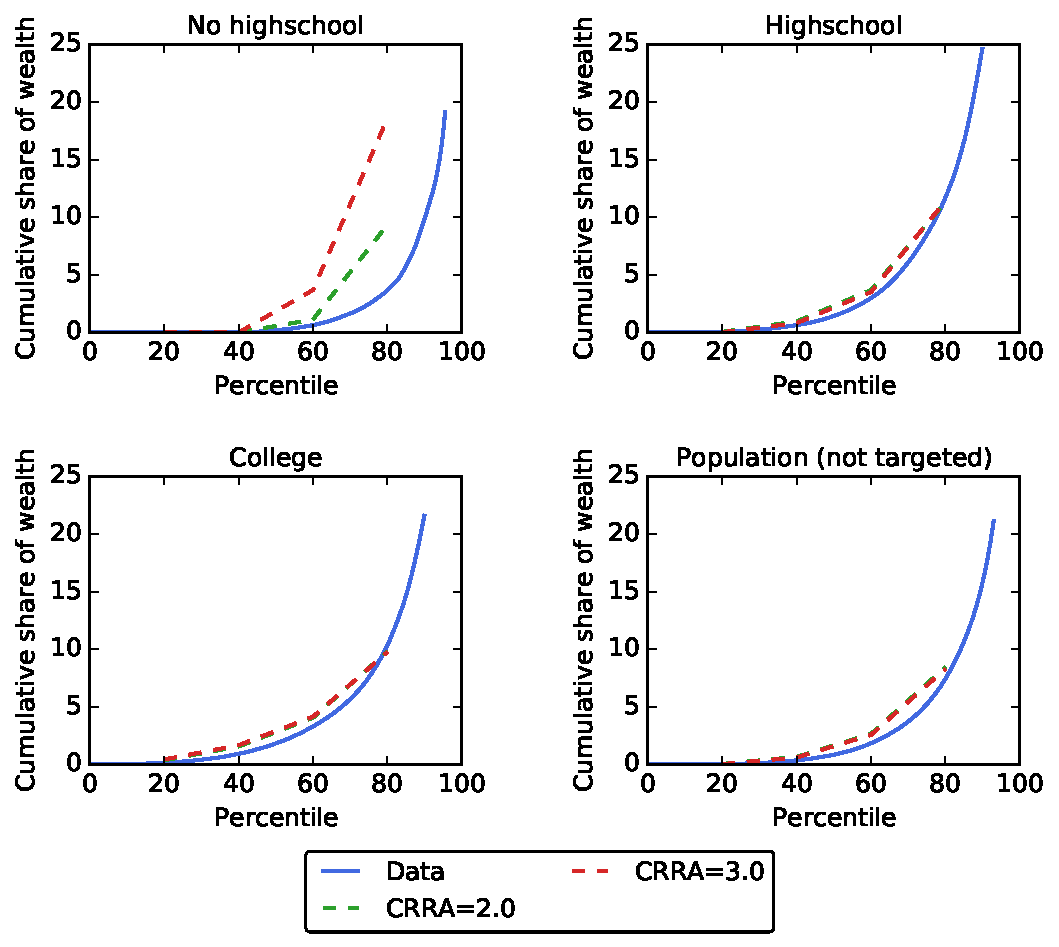
\includegraphics[width=.9\textwidth]{../Figures/LorenzPoints_robustness.pdf}
	\caption{Distributions of liquid wealth within each educational group and for the whole population from the 2004 Survey of Consumer Finance and from the estimated model for different values of risk aversion, $\gamma$.}
	\label{fig:LorenzPts_robustness}
\end{center}
\end{figure}

\subsubsection{Results with higher risk aversion}
\label{sec:robust_gamma_results}


\subsection{Altering the interest rate}
\label{sec:robust_R} 



\end{document}	